\documentclass[a4paper,oneside,12pt,titlepage]{article}
\usepackage[utf8]{inputenc}
\usepackage[français]{babel}
\usepackage{graphicx} % insertion images
\usepackage{hyperref}
\usepackage{amsmath}

\renewcommand*\contentsname{Table des matières}


\begin{document}

\begin{titlepage}
    \begin{center}
        \vspace*{1cm}
            
        \Huge
        \textbf{Projet de Programmation Avancée}
            
        \vspace{0.5cm}
        \LARGE
        Lancer de rayons
            
        \vspace{1.5cm}
            
        \textbf{Teddy ALEXANDRE, Arthur BABIN}
            
        \vfill
            
        \vspace{0.8cm}
            
        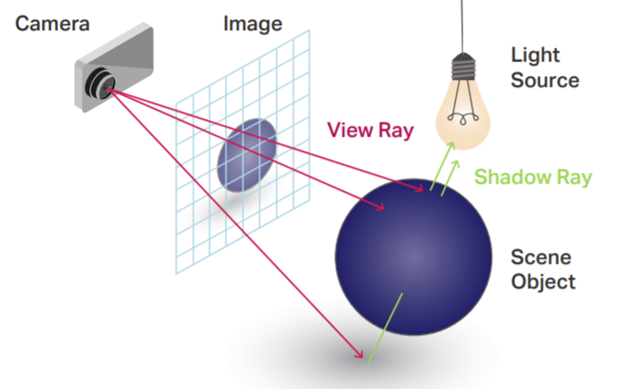
\includegraphics[width=\textwidth]{./raytracing_picture.png}

        \vfill
        \Large
        Décembre 2022
            
    \end{center}
\end{titlepage}

\tableofcontents
\newpage

\section{Introduction}

\begin{sloppypar}

Le sujet de notre projet de programmation avancée est le \textbf{lancer de rayons}. Il s’agit d’une technique de rendu de synthèse d’images 3D, c’est-à-dire d’obtention d’une scène d’objets en trois dimensions sur un écran en deux dimensions. Cette technique est très utilisée dans de nombreux domaines, notamment celui du jeu vidéo pour obtenir de bons rendus graphiques. \\[6pt]

Plusieurs techniques d’approches peuvent être employées, comme la \textbf{rastérisation}, qui consiste en l’application de formules de projection de l’image 3D en 2D. Le procédé est en général rapide mais parfois peu réaliste, car les ombres doivent être simulées. \\[6pt]

On utilise donc souvent une deuxième technique, plus réaliste, qui est le \textbf{tracé de rayons} (raytracing), et qui repose sur le principe du retour inverse de la lumière. En effet, au lieu de lancer des rayons à partir des diverses sources lumineuses pour voir où ils rebondissent, on part du point d’arrivée (la caméra dans le cadre du projet) et pour chaque pixel de l’écran, on observe la trajectoire du rayon lumineux dirigé vers ce pixel. La méthode est plus coûteuse en termes de temps d’exécution néanmoins, d’autant plus si on tient compte des diverses propriétés des matériaux des objets présents dans la scène (réflexivité, réfraction, transmission, etc.). \\[6pt]

C’est donc cette technique que nous avons dû mettre en place dans le cadre du projet. Ce dernier a été écrit en C++, commenté avec Doxygen, et utilise la bibliothèque externe SDL pour effectuer les affichages à l’écran.

\newpage

\section{Choix effectués}

\subsection{Modélisation du problème}

Nous avons fixé quelques conventions pour résoudre ce problème. On se place dorénavant dans l’espace (cf Figure \ref{fig:fig_rendu4}). \\[6pt]

La boîte englobante correspondant aux "murs" dans notre scène est de dimensions $(2000,1000,1000)$ et son centre est en $(0,500,0)$. Nous avons de plus placé la caméra en $(100,600,-400)$. 

En ce qui concerne la grille d’affichage de la scène, celle-ci se situe dans la direction $(0,0,200)$ par rapport à la caméra. De plus, l’origine du repère se situe en haut à gauche de la grille, avec l’axe des abscisses orienté vers la droite, et l’axe des ordonnées orienté vers le bas, conformément à la SDL qui fonctionne ainsi. \\[6pt]

Il y a également une source de lumière omnidirectionnelle presque au centre de la scène en $(100,500,0)$. Nous avons fait le choix de ne pas prendre en compte la direction de cette lumière pour un meilleur rendu mais on aurait également pu faire en sorte de pouvoir gérer une liste de lumières directionnelles et il aurait ainsi fallu prendre en compte pour chaque lumière le produit scalaire entre sa direction avec le vecteur unitaire partant du point d'intersection vers son origine.\\[6pt]

La scène dispose également d’une sphère et d’autres parallélépipèdes rectangles (alignés ou non par rapport aux axes) que l’on place librement dans la boîte, afin de vérifier le bon fonctionnement de l’algorithme de tracé de rayons.

\newpage

\subsection{Diagramme UML / Ajout de méthodes}

\begin{figure}[!h]
    \centering
    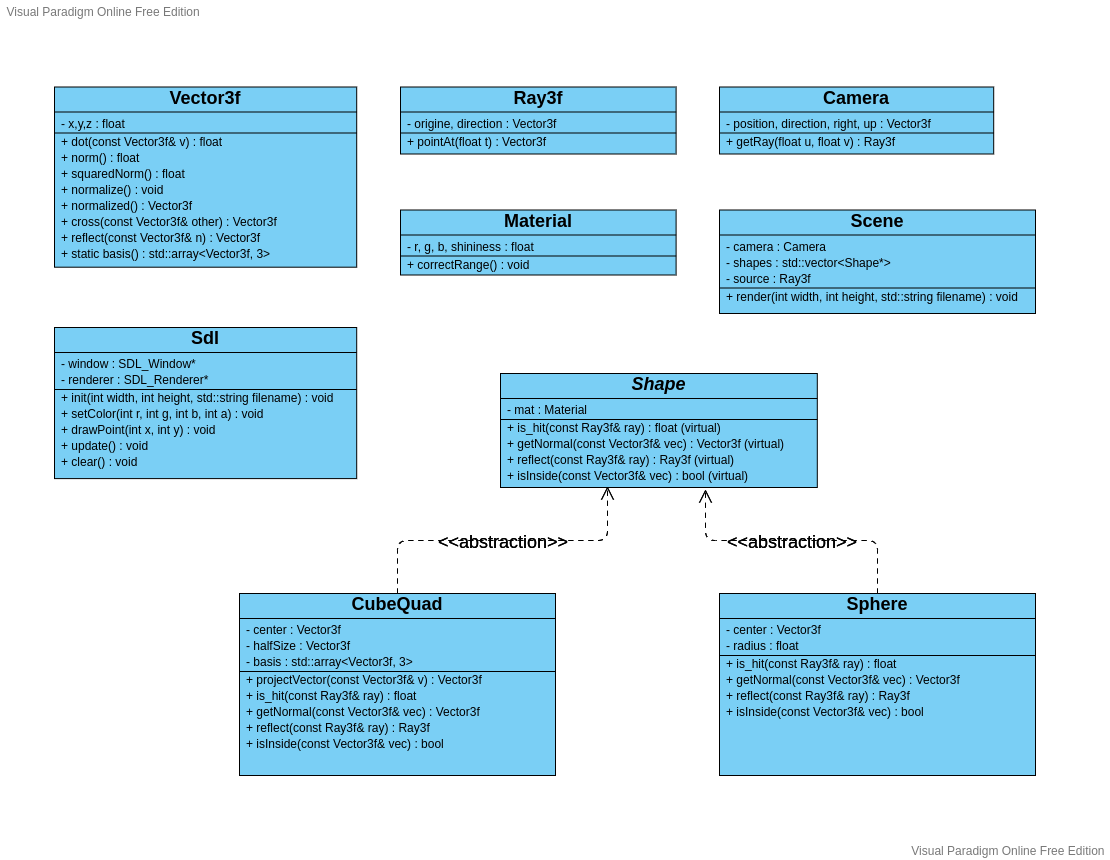
\includegraphics[width=\linewidth]{./Diagramme_UML.png}
    \caption{Diagramme UML du projet}
    \label{fig:uml}
\end{figure}

Nous avons fait le choix d’ajouter et de modifier quelques méthodes afin de faciliter certaines portions du code final. \\[6pt]

Dans la classe \textit{Vector3f}, des méthodes sur les calculs avec les vecteurs ont été ajoutées (produit scalaire, produit vectoriel, calcul de norme, normalisation d’un vecteur, vecteur réfléchi par rapport à un vecteur incident), elles servent essentiellement pour déterminer les intersections entre les objets et les rayons lumineux. \\[6pt]

Dans la classe \textit{Ray3f}, justement, nous avons ajouté une méthode pointAt qui détermine le point paramétré par un flottant $t$ sur la droite engendrée par le rayon lumineux (l'équation d'un rayon lumineux d'origine $O$ et de direction $\vec{d}$ étant $\overrightarrow{r(t)} = O + t\vec{d}$. \\[6pt]

Dans la classe abstraite \textit{Shape} (et donc ses classes filles \textit{CubeQuad} et \textit{Sphere}), on a surchargé la méthode \textit{is\_hit} en renvoyant la distance entre l’origine du rayon et la Shape si il y a intersection, -1 sinon. Nous avons également défini les méthodes \textit{getNormal} et \textit{isInside} qui déterminent respectivement le vecteur normal à la Shape en un point, et si un point se situe à l'intérieur de la Shape ou non. Ces deux méthodes virtuelles pures sont implémentées dans les classes filles \textit{CubeQuad} et \textit{Sphere}. \\[6pt] 

Dans \textit{CubeQuad}, nous avons modélisé les figures un peu différemment de l’énoncé : un cube est défini par son centre, sa \textbf{demi-taille} (sous forme de vecteur 3D), et la \textbf{base} dans laquelle le \textit{CubeQuad} est aligné par rapport aux axes. Cela nous permet ainsi d'afficher par exemple des cubes orientés. Nous avons aussi implémenté la base canonique associée aux \textit{CubeQuad} non orientés. \\[6pt]

On a enfin écrit une classe \textit{SDL} qui implémente des méthodes utiles de la bibliothèque SDL, afin d’en faciliter l’utilisation (masquage de l’utilisation des pointeurs sur la fenêtre et le rendu).

\newpage

\section{Calcul de la couleur d'un pixel}

Nous avons décidé d'utiliser un modèle de réflexion (additionné au modèle de Phong)(cf Figure \ref{fig:phong}) :
\begin{figure}[!h]
    \centering
    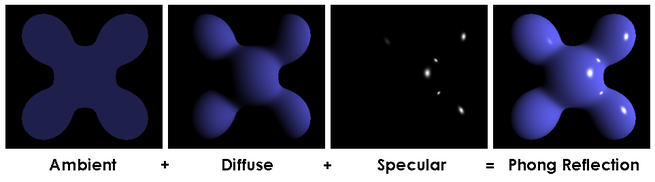
\includegraphics[width=\linewidth]{./Phong_components.png}
    \caption{Illustration du modèle de Phong : l'intensité totale est la somme des trois composantes décrites ci-dessus}
    \label{fig:phong}
\end{figure}

\begin{equation*}
  c_{\text{total}}^{\text{ray}} =
    \begin{cases}
      0 & \text{s'il n'y a pas d'intersection}\\
      c_{\text{a}} & \text{si le point d'intersection n'est pas éclairé}\\
      c_{\text{a}} + c_{\text{d}} + c_{\text{s}} + c_{\text{reflected}} & \text{sinon}\\
    \end{cases}\\
\end{equation*}
\begin{equation*}
  \text{avec}
    \begin{cases}
      s & \text{la shininess du matériau}\\
      \vec{n} & \text{la normale au point d'intersection}\\
      \vec{r} & \text{le vecteur unitaire intersection-lumière}\\
      c_{\text{material}} & \text{la couleur du matériau du point d'intersection}\\
      c_{\text{a}} = 0.2*c_{\text{material}} & \text{sinon}\\
      c_{\text{d}} = (\vec{n}\cdot\vec{r})c_{\text{material}} & \text{sinon}\\
      c_{\text{s}} = 0.1(\vec{n}\cdot\vec{r})^sc_{\text{material}}& \text{sinon}\\
      c_{\text{reflected}}=sc_{\text{total}}^{\text{reflected ray}} & \text{la couleur réfléchie}\\
    \end{cases}\\
\end{equation*}

\newpage

\section{Algorithmes et problèmes rencontrés}

Nous avons donc suivi l’algorithme fourni dans l’énoncé : la détermination de la grille n’a pas posé de problème particulier. \\[6pt] 

Concernant le calcul de l’image, plusieurs problèmes se sont posés :
\begin{itemize}
    \item Comment gérer les intersections pour calculer le rayon réfléchi ? Comment alors gérer le cas d’une réflexion (objet avec coefficient de luminosité strictement positif) ?
\end{itemize}


En effet, afin de déterminer entièrement le rayon réfléchi, nous avons besoin de connaître le point d’intersection entre le rayon incident et notre objet (cube ou sphère). En fonction du type de primitive, on peut alors déterminer le vecteur normal et en déduire le rayon incident. C’est donc ainsi que nous avons implémenté pour chaque primitive une méthode reflect qui calcule ce rayon réfléchi r, dont la formule est donnée grâce aux lois de Descartes sur la réflexion et la réfraction : \\[2pt] 

$\vec{r} = \vec{i} - 2(\vec{i} \cdot \vec{n})\vec{n}$, avec $\vec{i}$ le rayon incident et $\vec{n}$ le vecteur normal. \\[2pt] 

On peut donc implémenter les réflexions pour calculer les couleurs, en écrivant un programme récursif pour le faire de la manière la plus naturelle possible.

\begin{itemize}
    \item Comment savoir si un pixel est caché ou pas ? Comment calculer alors la couleur finale d’un pixel ?
\end{itemize}

Afin de déterminer comment colorier le pixel, on a besoin de savoir si le point associé dans la scène est exposé à la source de lumière. Nous avons donc parcouru l’ensemble des primitives de la scène, et vérifié si chacune des primitives était frappé par le rayon qui part du point d’intersection entre le rayon incident et l’objet, et qui se dirige vers la source de lumière. Si c’est le cas, le pixel est caché et l’on affiche avec un gris sombre (afin de distinguer du noir complet, de la couleur de fond). Sinon on utilise les propriétés de notre Shape, et notamment de son Material pour renvoyer une couleur au format RGB. On peut bien évidemment complexifier l’ensemble et introduire un coefficient de réflexion pour tenir compte des réflexions sur l’objet, qui contribuent aussi à la couleur finale du pixel.\\[6pt]

En ce qui concerne les pavés droits orientés c'est-à-dire non alignés par rapport aux axes nous avons ajouté un attribut \textit{basis} qui correspond à la base de vecteurs dans laquelle le \textit{CubeQuad} est aligné. Cet attribut nous permet ainsi d'utiliser les algorithmes d'intersection d'une droite avec des plans lorsqu'ils sont alignés par rapport aux axes après une projection du rayon dans la base correspondante. Cependant nous avons rencontré un problème que nous n'avons pas su résoudre: la position des \textit{CubeQuad} orientés subit une translation non désirée et non constante (elle dépend de l'angle de rotation) mais cela n'a pas de répercussion sur la qualité ou le réalisme du rendu.

\newpage

\section{Réalisation et rendu final}

Le rendu final est fonctionnel, avec un programme qui compile et un affichage sur la fenêtre créée avec la classe SDL. Nous avons réussi, par le biais d’une fonction récursive, à rajouter les effets de la réflexion en fonction de la luminosité. Bien que le temps d'exécution soit rallongé à cause des calculs récursifs (de l'ordre d'une dizaine de secondes), les rendus restent très appréciables de ce point de vue là. \\[6pt] 

Néanmoins, tout n’est pas parfait : la présence de petits points au niveau des figures donne un rendu parfois un peu brouillon, ce qui est aussi accentué par la présence d’aliasing à l’écran (les images sont crénelées). Il était donc possible d’aller plus loin dans le projet à ce niveau-là. \\[6pt] 

En effet, nous n'avons pas pu consacrer suffisamment de temps au projet, qui aurait pu être encore plus travaillé et offrir donc un meilleur rendu. L’ensemble était néanmoins difficile à conjuguer avec les cours en parallèle et les autres projets à rendre. \\[6pt] 

Nous sommes satisfaits de pouvoir obtenir un rendu d’image 3D avec l’ensemble des classes implémentées, car cela a tout de même requis un certain temps avant de pouvoir afficher des rendus intéressants à la fenêtre.


\section{Conclusion sur le projet}

Le projet de tracé de rayons s’est révélé très intéressant, et nous a permis d’en apprendre davantage sur les méthodes de rendu d’images 3D grâce aux théorèmes d’optique. Il nous a permis également de renouer avec quelques théorèmes et fondements de l’optique, qui ont été abordés antérieurement dans notre formation d’ingénieur (en prépa scientifique plus précisément), ainsi que quelques calculs géométriques. \\[6pt] 

Ce projet nous a également permis de nous convaincre de l’intérêt certain que possède la programmation orientée objet, qui s’est révélée très utile ici. Nous ne sommes pas certains que ce projet aurait été plus simple sans l’apport de ce paradigme de programmation. 


\begin{figure}[!h]
    \centering
    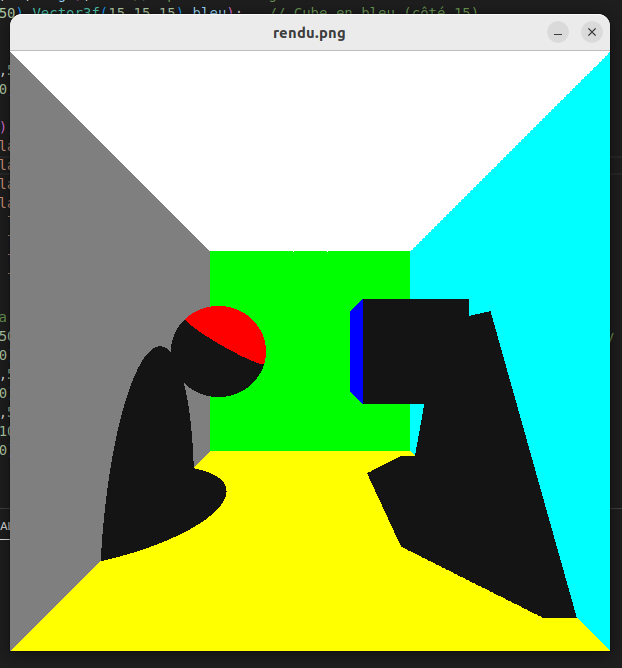
\includegraphics[width=\linewidth]{./premier_rendu.png}
    \caption{Premier rendu obtenu, sans les réflexions et sans dégradé de couleur}
    \label{fig:fig_rendu1}
\end{figure}

\begin{figure}[!h]
    \centering
    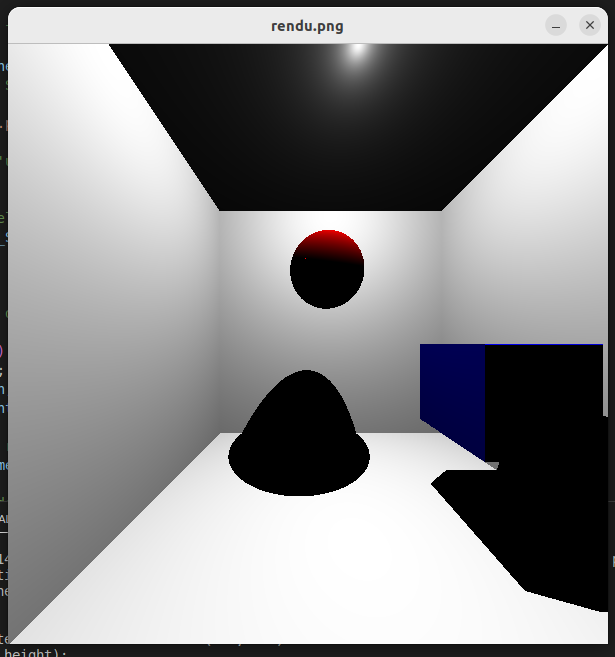
\includegraphics[width=\linewidth]{./deuxieme_rendu.png}
    \caption{Second rendu obtenu, avec un dégradé de couleur suivant l'angle d'inclinaison avec la source de lumière}
    \label{fig:fig_rendu2}
\end{figure}

\begin{figure}[!h]
    \centering
    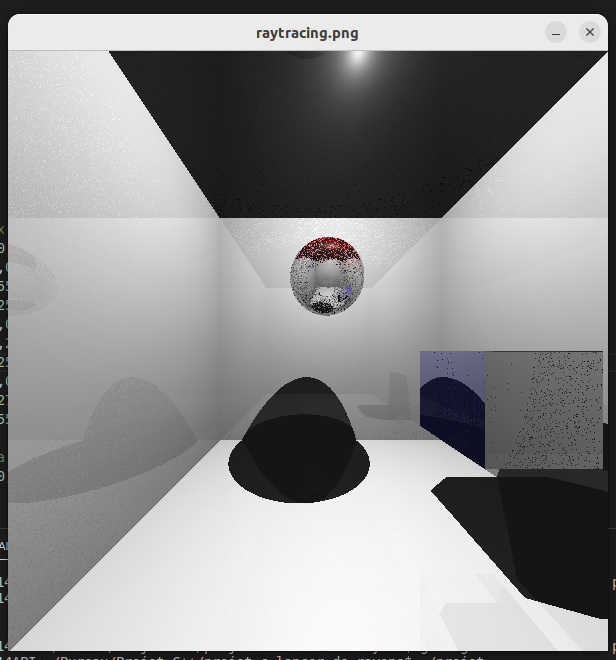
\includegraphics[width=\linewidth]{./rendu_reflexions.png}
    \caption{Rendu avec des effets de réflexion sur les objets}
    \label{fig:fig_rendu3}
\end{figure}

\begin{figure}[!h]
    \centering
    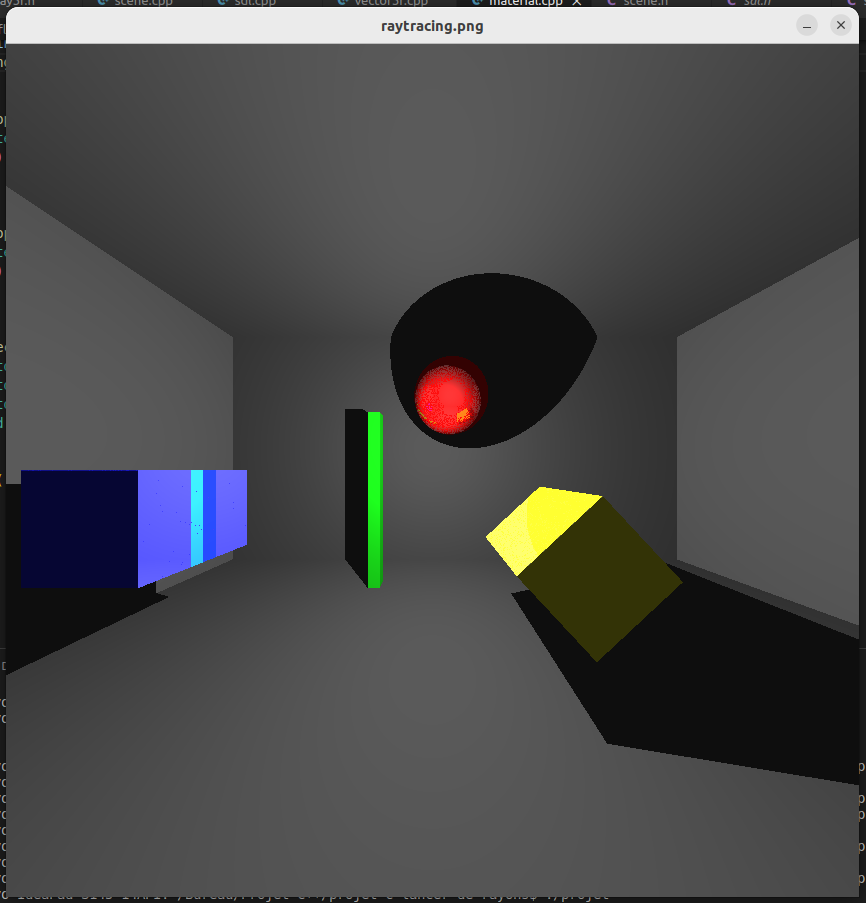
\includegraphics[width=\linewidth]{./rendu_modele_phong.png}
    \caption{Rendu obtenu en appliquant le modèle de Phong}
    \label{fig:fig_rendu4}
\end{figure}

\begin{figure}[!h]
    \centering
    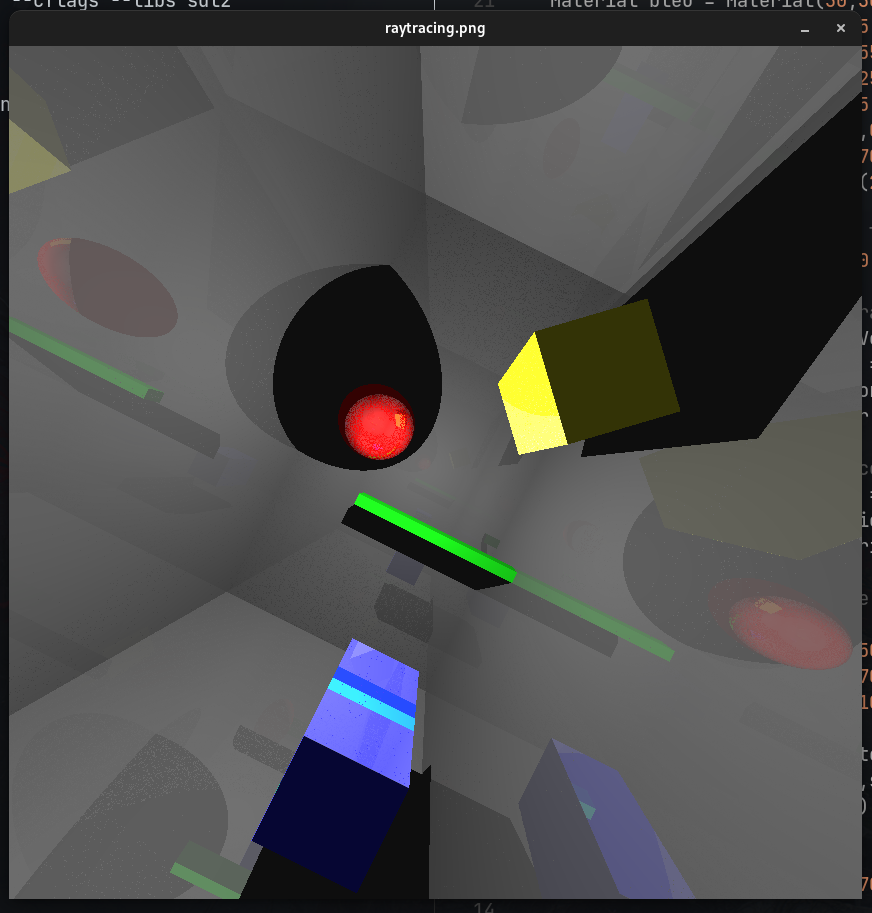
\includegraphics[width=\linewidth]{./rendu_modele_phong2.png}
    \caption{Rendu obtenu en appliquant le modèle de Phong (avec rotation de la caméra et des murs légèrement réfléchissants)}
    \label{fig:fig_rendu5}
\end{figure}

\end{sloppypar}

\end{document}
